\documentclass{article}
\usepackage[T2A]{fontenc}
\usepackage{float}
\usepackage{geometry}
\geometry{
	a4paper,
	top=25mm, 
	right=15mm, 
	bottom=25mm, 
	left=30mm
}


\usepackage{graphicx} % Required for inserting images
\usepackage{amsmath}
\usepackage[english,russian]{babel}

\title{Работа 1.1.1\\ 
	Определение систематических и случайных погрешностей при измерении удельного сопротивления нихромовой проволоки}


\begin{document}
	
	\maketitle
	
	\section{Аннотация}
	В работе измеряется удельное сопротивление нихромовой проволоки двумя способами: 1) путем анализа графика ВАХ проволоки, 2) путем вычисления по известной формуле \(R = \rho \frac{l}{S}\), где \( R\) измерено  посредством моста Уильсона (моста постоянного тока).\\\\
	\emph{Цель работы:} измерение удельного соединения нихромовой проволоки и вычисление систематических и случайных погрешностей при использовании измерительных прибров. \\\\
	\emph{Оборудование:} линейка, штангенциркуль, микрометр, нихромовая проволока, амперметр, стрелочный вольтметр, источник ЭДС, мост Уильсона (мост постоянного тока), реостат, ключ, провода.
	
	\section{Теоретические сведения}
	
	Удельное сопротивление цилиндрической проволоки определяется по формуле:
	$ \rho = \frac{R}{l}S $, а учитывая что $ S = {\pi}{\frac{d^2}{4}} $,
	
	$$ \rho = \frac{R}{l}{\frac{{\pi}d^2}{4}} $$
	Где $ R $ - сопротивление отрезка проволоки, $ l $ - его длина, $ d $ - диаметр.\\\\
	По закону Ома для участка цепи: 
	$$ R = \frac{U}{I} $$
	$ U $ - напряжение на участке цепи, $ I $ - сила тока, $ R $ - сопротивление.\\
	
	Таким образом, для определения сопротивления проволоки достаточно измерить силу тока и напряжение на нем. Это возможно с помощью схемы рис.1.\\
	\begin{figure}
		\centering
		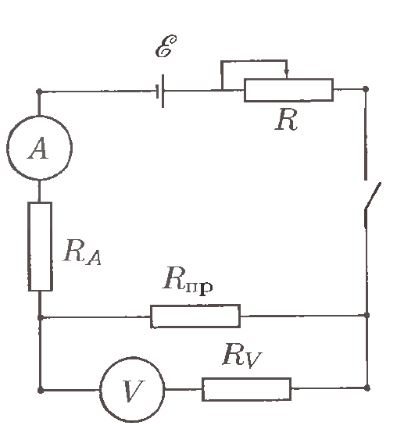
\includegraphics[width = 0.5\linewidth]{1.png}
		\caption{Используемая схема}
		\label{fig:enter-label}
	\end{figure}
	
	Вольтметр верно измеряет падение напряжения на проволоке, а амперметр измеряет сумму токов через проволоку и вольтметр. Поэтому можно записать систему:\\
	\begin{equation}
		\begin{cases}
			$$ I_{A} = I + I_{V} $$\\
			$$IR = U_{V} $$\\
			$$I_{V}R_{V} = U_{V} $$
		\end{cases} 
	\end{equation}
	$U_{V}$ - показания вольтметра, $I_{A}$ - показания амперметра\\\\
	Выразив токи $I$ и $I_{V}$ и подставив их в первое уравнение получим\\
	\begin{equation}
		\label{R_fake}
		R_{\text{1}} = \frac{U_{V}}{I_{A}}= R\frac{R_{V}}{R+R_{V}}
	\end{equation}
	Здесь $R_{1}$ не является истинным сопротивлением проволоки, выразим истинное сопротивление $R$ из (\ref{R_fake}):
	
	$$R = \frac{R_{1}}{1 - \frac{R_{1}}{R_{V}}}$$
	В силу величины $R_{V}$ по сравнению с $R_{1}$:
	
	\begin{equation}
		R \approx R_{1}(1 + \frac{R_{1}}{R_{V}})
	\end{equation}
	
	
	
	\section{Оборудование и экспериментальные погрешности}
	
	\emph{Линейка}: $\Delta_{\text{лин}} = \pm 0.5$ мм (половина цены деления)\\
	\emph{Штангенциркуль}: $\Delta_{\text{шт}} = \pm 0.05$ мм (половина цены деления)\\
	\emph{Микрометр}: $\Delta_{\text{мкм}} = \pm 0.01$ мм (маркировка производителя)\\
	\emph{Амперметр}: $\Delta_{\text{А}} = \pm (0.002 * X + 2k)$, где X - измеряемая величина, k - единица младшего разряда (k = 0.01 мА) (согласно паспорту прибора)\\
	\emph{Вольтметр}: $\Delta_{\text{V паспорт}} = \pm (0.005 * X)$, где X - измеряемая величина (согласно классу точности)\\
	Т.к. положение стрелки вольтметра определялось на глаз, к погрешности вольтметра можно прибавить половину цены деления :\\
	
	$$\Delta_{\text{V}} = \pm (0.005 * X + 0.5 * c),$$ где c - цена деления\\
	
	Т.к. $R_{V}(U_{V}, I_{V}) = \frac{U_{V}}{I_{V}}$, имеем 
	\[\sigma_{R_{V}} = \sqrt{ (\frac{\delta R_{V}}{\delta U_{V}}\Delta_{V})^{2} + (\frac{\delta R_{V}}{\delta I_{V}}\Delta_{A})^{2} }\]
	
	\[\sigma_{\text{сист}R_{1}} = \sqrt{ (\frac{\Delta_{V}}{I_{V}})^{2} + (\frac{U_{V}}{I_{V}^{2}}\Delta_{A})^{2} }\]
	
	Получаем $$\sigma_{R_{V}} = 0,0275 ~\Omega$$
	$$R_{V} = \frac{600}{0.15} = 4000 ~\Omega $$
	(согласно маркировке при $U_{V} = 600$ В. $I_{V} = 0.15$ А)\\
	
	По сравнению с $R_{V}$, $\sigma_{R_{V}}$ слишком мала, поэтому ей можно пренебречь:
	
	$\sigma_{R_{V}} \approx 0 ~\Omega$\\
	\emph{Мост постоянного тока Р4833}:\\
	Класс точности: 0,1\\
	Разрядность магазина сопротивлений: 5 ед.\\
	Используемый множитель: $10^{-1}$\\
	Погрешность измерений в используемом диапазоне: $\Delta_{\text{мост}} = \pm 0,0001 ~\Omega$.\\
	
	
	\section{Измерения и обработка данных}
	
	\subsection{Измерение длины проволоки $l$}
	Значения $l$ измерялись с помощью линейки.\\
	$\Delta_{\text{l}} = 2\Delta_{\text{лин}} = \pm 1\text{ мм}$ (т.к. оба конца проволоки не были зафиксированы)
	
	\subsection{Измерение диаметра проволоки $d$}
	Проволока неоднородна, поэтому ее диаметр различен в разных местах. Мы можем измерить его в нескольких местах и усреднить полученные значения.\\\\
	Измерения с помощью штангенциркуля показали одинаковый диаметр проволоки для $N = 12$ измерений, $d_{\text{шт}} = 0.4 \text{мм}$.\\
	
	\begin{table}[H]
		\centering
		\begin{tabular}{|c|c|c|c|c|c|c|c|c|c|c|c|c|}
			\hline
			№ & 1 & 2 & 3 & 4 & 5 & 6 & 7 & 8 & 9 & 10 & 11 & 12 \\ \hline
			$d_{\text{шт}}$, мм & 0.4 & 0.4 & 0.4 & 0.4 & 0.4 & 0.4 & 0.4 & 0.4 & 0.4 & 0.4 & 0.4 & 0.4 \\ \hline
		\end{tabular}
		\caption{Результат измерения $d$ штангенциркулем}
	\end{table}
	Для измерения диаметра был также использован микрометр, который выявил отличия в диаметре проволоки в разных ее местах (см. Табл. 1).
	
	\begin{table}[H]
		
		\centering
		\begin{tabular}{|c|c|c|c|c|c|c|c|c|c|c|c|c|}
			\hline
			№ & 1 & 2 & 3 & 4 & 5 & 6 & 7 & 8 & 9 & 10 & 11 & 12 \\ \hline
			$d_{\text{мкм}}$, мкм & 380 & 380 & 360 & 390 & 360 & 370 & 350 & 340 & 360 & 380 & 370 & 370 \\ \hline
		\end{tabular}
		\caption{Результат измерения $d$ микрометром}
	\end{table}
	Средний диаметр $$\overline{d} = \frac{\Sigma d_{i}}{N} = 367.5 \text{ мкм}$$\\
	Среднее квадратичное отклонение $$\sigma_{d} = \sqrt{\frac{1}{N}\sum_{i = 1}^{N} \Delta d^{2}_{i}} = 13.62 \text{ мкм}$$\\
	Погрешность среднего $$\sigma_{\overline{d}} = \frac{\sigma_{d}}{\sqrt{N}} = 3.93 \text{ мкм}$$
	Общая погрешность $$\sigma_{d} = \sqrt{\sigma_{\overline{d}}^{2} + \Delta_{\text{мкм}}^{2}} = 10.74 \text{ мкм} \approx 10.7 \text{ мкм}$$\\
	
	Следовательно,\\
	$$d = (367.5 \pm 10.7) \text{ мкм}$$\\
	
	
	\subsection{Вычисление сопротивления проволоки $R$}
	Измерить сопротивление отрезка проволоки $R$ возможно двумя способами
	
	\subsubsection{Вычисление $R$ путем анализа ВАХ проволоки}
	Для снятия ВАХ проволоки была собрана схема Рис. 1\\
	ВАХ снималась для трех разных длин проволоки путем постепенного уменьшения напряжения источника. Результаты измерений приведены в Табл. 3, 4, 5.
	\\
	
	
	\begin{table}[H]
		\centering
		\begin{tabular}{|c|c|c|c|c|}
			\hline
			№ & Uист, В & Uv, дел & Uv, мВ & Ia, мА \\ \hline
			1 & 3.5 & 148 & 592 & 111.16 \\ \hline
			2 & 3.3 & 137 & 548 & 103.42 \\ \hline
			3 & 3.1 & 130 & 520 & 97.84 \\ \hline
			4 & 2.9 & 121 & 484 & 90.41 \\ \hline
			5 & 2.7 & 115 & 460 & 86.6 \\ \hline
			6 & 2.3 & 98 & 392 & 73.78 \\ \hline
			7 & 1.9 & 80 & 320 & 60.3 \\ \hline
			8 & 1.5 & 64 & 256 & 47.9 \\ \hline
			9 & 1.1 & 36 & 144 & 26.63 \\ \hline
			10 & 0.7 & 23 & 92 & 17.29 \\ \hline
			11 & 0.2 & 3 & 12 & 1.98 \\ \hline
		\end{tabular}
		\caption{ВАХ проволоки $l = (500.0 \pm 0.5)$ мм}
	\end{table}
	
	\begin{table}[H]
		\centering
		\begin{tabular}{|c|c|c|c|c|}
			\hline
			№ & Uист, В & Uv, дел & Uv, мВ & Ia, мА \\ \hline
			1 & 3.5 & 150 & 600 & 184.86 \\ \hline
			2 & 3.3 & 143 & 572 & 176.44 \\ \hline
			3 & 3.1 & 136 & 544 & 167.57 \\ \hline
			4 & 2.9 & 124 & 496 & 152.78 \\ \hline
			5 & 2.7 & 118 & 472 & 145.04 \\ \hline
			6 & 2.3 & 100 & 400 & 123.58 \\ \hline
			7 & 1.9 & 84 & 336 & 103.16 \\ \hline
			8 & 1.5 & 67 & 268 & 82.66 \\ \hline
			9 & 1.1 & 48 & 192 & 59.25 \\ \hline
			10 & 0.7 & 21 & 84 & 25.31 \\ \hline
			11 & 0.2 & 2 & 8 & 1.79 \\ \hline
		\end{tabular}
		\caption{ВАХ проволоки $l = (300.0 \pm 0.5)$ мм}
	\end{table}
	
	\begin{table}[H]
		\centering
		\begin{tabular}{|c|c|c|c|c|}
			\hline
			№ & Uист, В & Uv, дел & Uv, мВ & Ia, мА \\ \hline
			1 & 3.5 & 149 & 596 & 271.1 \\ \hline
			2 & 3.3 & 139 & 556 & 256.15 \\ \hline
			3 & 3.1 & 130 & 520 & 241.29 \\ \hline
			4 & 2.9 & 123 & 492 & 227.4 \\ \hline
			5 & 2.7 & 112 & 448 & 208.09 \\ \hline
			6 & 2.3 & 98 & 392 & 181.76 \\ \hline
			7 & 1.9 & 80 & 320 & 147.89 \\ \hline
			8 & 1.5 & 64 & 256 & 118.08 \\ \hline
			9 & 1.1 & 47 & 188 & 87.3 \\ \hline
			10 & 0.7 & 16 & 64 & 29.91 \\ \hline
			11 & 0.2 & 6 & 24 & 10.65 \\ \hline
		\end{tabular}
		\caption{ВАХ проволоки $l = (200.0 \pm 0.5)$ мм}
	\end{table}
	
	1 дел = $\frac{600 \text{ мВ}}{150 \text{ дел}}$ = 4 мВ\\
	
	Построим график U(I) по данным Табл.3, 4, 5: угловые коэффициенты $k_{20}, k_{30}, k_{50}$ этих прямых будут соответствовать величинам соответствующих ${R_{1}}$ 
	
	
	\begin{figure}[H]
		\centering
		\rotatebox{90} {
			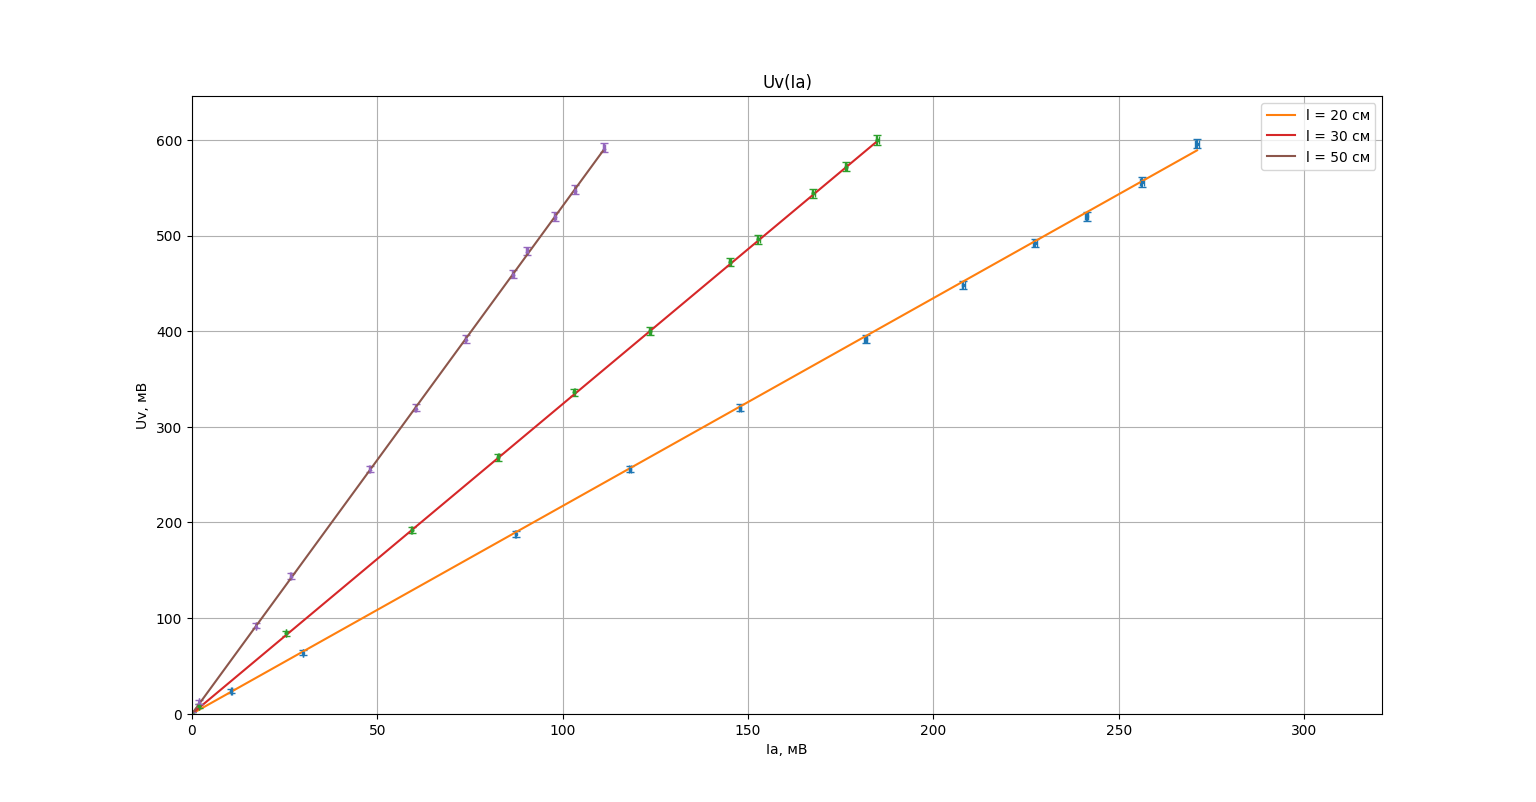
\includegraphics[width = 1.4\linewidth]{Figure_2.png}}
		\caption{Прямые $U_{V}(I_{A})$ \text{для трех значений l}}
		\label{fig:enter-label}
	\end{figure}
	
	Систематическую погрешность $R_{1}$ оценим как ошибку косвенного измерения по максимальным систематическим погрешностям $\Delta_{A}$ и $\Delta_{V}$.\\  
	Т.к. $R_{1}(U_{V}, I_{A}) = \frac{U_{V}}{I_{A}}$, имеем систематическую погрешность
	\[\sigma_{\text{сист}R_{1}} = \sqrt{ (\frac{\delta R_{1}}{\delta U_{V}}\Delta_{V})^{2} + (\frac{\delta R_{1}}{\delta I_{A}}\Delta_{A})^{2} }\]
	
	\[\sigma_{\text{сист}R_{1}} = \sqrt{ (\frac{\Delta_{V}}{I_{A}})^{2} + (\frac{U_{V}}{I_{A}^{2}}\Delta_{A})^{2} }\]
	
	Систематическую погрешность $\sigma_{\text{сист}R_{1}}$ берем максимальную для всех измерений каждого $l$.
	$$\sigma_{\text{полн}R_{1}} = \sqrt{\sigma_{\text{случ}R_{1}}^{2} + \sigma_{\text{сист}R_{1}}^{2}}$$
	
	
	\begin{table}[H]
		\centering
		\begin{tabular}{|c|c|c|c|c|}
			\hline
			l, см & $R_{1}$, ом & $\sigma_{\text{случ}R_{1}}, \Omega$ & $\sigma_{\text{сист}R_{1}}, \Omega$ & $\sigma_{\text{полн}R_{1}}, \Omega$ \\ \hline
			50 & 5.32066 & 0.00611 & 1.04299 & 1.04591 \\ \hline
			30 & 3.24624 & 0.00260 & 1.14118 & 1.14232 \\ \hline
			20 & 2.16850 & 0.00488 & 0.19925 & 0.21114 \\ \hline
		\end{tabular}
		\caption{Определение $R_{1}$ по графику $U(I)$}
	\end{table}
	
	В итоге,\\
	для $l = (500 \pm 0.5$) мм 
	$$R_{1} = (5.32066 \pm 1.04591) \Omega$$\\
	для $l = (300 \pm 0.5$) мм 
	$$R_{1} = (3.24624 \pm 1.14232) \Omega$$ \\
	для $l = (200 \pm 0.5$) мм 
	$$R_{1} = (2.16850 \pm 0.21114) \Omega$$ \\
	
	Найдем $R$ по формуле (3). 
	Погрешность косвенной величины $R$:
	
	$$\sigma_{R} = \sqrt{(2\frac{R_{1}}{R_{V}} + 1)^{2} \sigma_{R_{1}}^{2} + (R_{1} - \frac{R_{1}}{R_{V}^{2}})^{2} \sigma_{R_{V}}^{2}}$$
	
	Т.к. $\sigma_{R_{V}} \approx 0$, получаем
	
	$$\sigma_{R} = (2\frac{R_{1}}{R_{V}} + 1) \sigma_{R_{1}}$$
	
	
	\begin{table}[H]
		\centering
		\begin{tabular}{|c|c|c|}
			\hline
			l, см & $R, ~\Omega$ & $\sigma_{R}, ~\Omega$ \\ \hline
			50 & 5,328 & 1,049 \\ \hline
			30 & 3,249 & 1,144  \\ \hline
			20 & 2,170 & 0,211 \\ \hline
		\end{tabular}
		\label{RRR}
		\caption{Вычисление R}
	\end{table}
	
	
	
	\subsubsection{Прямое измерение $R$ с помощью моста постоянного тока}
	Для измерения $R$ использовался мост постоянного тока Р4833. Т.к. $\Delta_{\text{мост}} = \pm 0,0001 ~\Omega $ << значений Табл 7., будем считать $\Delta_{\text{мост}} = 0 ~\Omega$. Для трех $l$ были подобраны такие положения рубильников, при котором стрелка прибора была минимально отклонена от нуля.\\
	\begin{table}[H]
		\centering
		\begin{tabular}{|c|c|c|}
			\hline
			l, м & $R, ~\Omega$ & $\Delta{\text{мост}}, ~\Omega$ \\ \hline
			0.5 & 5.3 & 0.0001 \\ \hline
			0.3 & 3.235 & 0.0001 \\ \hline
			0.2 & 2.121 & 0.0001 \\ \hline
		\end{tabular}
		\caption{Измерение $R$ на мосте постоянного тока}
	\end{table}
	
	
	
	\subsection{Вычисление $\rho_{\text{уд}}$}
	\subsubsection{Для метода вычисления $R$ путем анализа ВАХ проволоки}
	$$ \rho = \frac{R}{l}{\frac{{\pi}d^2}{4}} $$
	
	$$\sigma_{\rho} = \sqrt{(\frac{\pi d^{2}}{4l} \sigma_{R})^{2} +
		(\frac{\pi d}{2l} \sigma_{d})^{2} +
		(\frac{\pi d^{2}}{4l^{2}} \Delta_{l})^{2}}$$
	
	\begin{table}[H]
		\centering
		\begin{tabular}{|c|c|c|}
			\hline
			l, м & $\rho, \frac{\Omega \text{мм}^{2}}{\text{м}}$ & $\sigma_{\rho}, \frac{\Omega \text{мм}^{2}}{\text{м}}$ \\ \hline
			0.5 & 1.13026 & 0.23201 \\ \hline
			0.3 & 1.14873 & 0.40456 \\ \hline
			0.2 & 1.15072 & 0.11214 \\ \hline
		\end{tabular}
		\caption{Вычисление $\rho_{\text{уд}}$}
	\end{table}
	
	Усредняя результаты 3-х опытов окончательно получаем:
	$$\rho_{\text{уд}} = 1.14323 \pm 0.24957 ~\frac{\Omega ~\text{мм}^{2}}{\text{м}} (\epsilon_{\rho} = 21.8 \%)$$
	
	\subsubsection{Для метода прямого измерения $R$ с помощью моста постоянного тока}
	
	$$ \rho = \frac{R}{l}{\frac{{\pi}d^2}{4}} $$
	
	$$\sigma_{\rho} = \sqrt{(\frac{\pi d^{2}}{4l} \Delta{\text{мост}})^{2} +
		(\frac{\pi d}{2l} \sigma_{d})^{2} +
		(\frac{\pi d^{2}}{4l^{2}} \Delta_{l})^{2}}$$
	
	\begin{table}[H]
		\centering
		\begin{tabular}{|c|c|c|}
			\hline
			l, м & $\rho, \frac{\Omega \text{мм}^{2}}{\text{м}}$ & $\sigma_{\rho}, \frac{\Omega \text{мм}^{2}}{\text{м}}$ \\ \hline
			0.5 & 1.12437 & 0.065480 \\ \hline
			0.3 & 1.14382 & 0.001907 \\ \hline
			0.2 & 1.12490 & 0.002813 \\ \hline
		\end{tabular}
		\caption{Вычисление $\rho_{\text{уд}}$}
	\end{table}
	
	Усредняя результаты 3-х опытов окончательно получаем:
	$$\rho_{\text{уд}} = 1.13103 \pm 0.02340 ~\frac{\Omega ~\text{мм}^{2}}{\text{м}} (\epsilon_{\rho} = 2 \%)$$
	
	К сожалению, использовать этот результат мы не можем т.к. проволока была откручена, а потом снова прикручена, что нарушило эксперимент. В окончательный ответ попадает значение из метода анализа ВАХ проволоки.
	
	\section{Вывод}
	
	Однажды Эрнест Хемингуэй поспорил, что затехает лабу 1.1.1 за 5 часов. Он проспорил. 
	В результате были измерены $R$ нихромовой проволоки для 3 ее длин, и по этим данным было вычислено $$\rho_{\text{уд. нихрома}} = 1.14323 \pm 0.24957 ~\frac{\Omega ~\text{мм}^{2}}{\text{м}} (\epsilon_{\rho} = 21.8 \%)$$
	
	Еще Эрнест Хемингуэй открутил проволоку и заруинил вторую часть эксперимента, но он был уверен, что если бы он это не сделал, все бы отлично сошлось.
	
	Когда мою лабу увидел оксимирон, он спел:\\\\ 
	\textit{Практически готов идеальный финал (Да-да-да-да-да)\\
		До смешного близок мечтаний предел (Да-да-да-да-да)\\
		Оправдана уйма стараний и сил\\
		Неизбежно верен счастливый прогноз...}\\\\
	Надеюсь следующие лабы пойдут быстрее, а то 13 часов это какой-то ужас. 
	
	
\end{document}
